
El desarrollo de software es un proceso iterativo, no es un producto con un inicio de fabricación y un fin; evoluciona. El final de un proyecto de software es cuando se deja de utilizar o mantener. La tecnología evoluciona y el software ha de evolucionar con ella o comienza un proceso de degradación de el producto, que si bien puede considerarse como la amortización de cualquier maquinaria, en el software ocurre a mayor velocidad. Por lo tanto el mismo diseño del software debe estar enfocado para soportar cambios y garantizar que la estructura del código no obstaculice dicho proceso iterativo.

Las definiciones más puras de los procesos de creación de software según Agile van enfocados a cero documentación y cero diseño. Sin embargo, es inevitable una primera toma de requisitos del cliente y la propuesta inicial para la toma de decisiones a la hora de invertir recursos. Este diseño inicial es planteado ya directamente como un producto minimo viable MVP y que el mismo software actue como dicha presentación. Sin embargo, tanto por el formato del trabajo como por opinión profesional de caracter personal, se va a hacer el ejercicio de utilizar el formato de un proyecto de tipo industrial para la entrega de dicha presentacion. El proceso iterativo de toma de requisitos mínimos y aceptación por parte del cliente es un punto vital. No sólo puede llegar a ser inevitable, si no que creo inconveniente eludir. Añade garantías a la seguridad de los responsables de la ejecución, de su exito comercial. El cliente muchas veces también quiere garantías de que se ha entendido sus requerimientos antes de dedicar recursos al proyecto. Una mínima base de acuerdo y comprensión documentada antes de abarcar un trabajo evita malos entendidos y frustraciones económicas. Todo euro gastando en diseño supone un ahorro sustancial en la ejecución.

Vamos a analizar la conveniencia de la combinación de dicha documentación inicial y usar una metodología ágil para evitar la parálisis por análisis. En el software conviene no centrarse en detalles técnicos que deben investigarse, analizarse o ponerse a prueba con su propia implementación. El proyecto ejecutivo inicial se entregará como un documento explicativo del diseño, con un equilibrio entre el detalle para eliminar incertidumbre y la pragmatismo de no crear una documentación excesiva condenada a quedar desactualizada en cuanto se ponga en marcha el proceso de desarrollo.

Se van a concretar los aspectos que se sean núcleo mismo del problema que se quiere resolver y señalar los puntos de incertidumbre, pero no será la documentación de una solución cerrada. En un proyecto real el presupuesto indicará hasta dónde se puede resolver dicha incertidumbre. Aunque el presupuesto se agotara, el programa debe entregarse, ser válido y funcional a nivel de lógica de negocio; únicamente pendiente de resolver la parte afectada para no malgastar recursos. En el lenguaje que vamos a desarrollar se definiría como: dejar el dominio definido, los casos de uso de la capa de aplicación desarrollados y, si no se consigue despejar la incertidumbre tecnológica, dejar únicamente pendiente de resolver los adaptadores que cumplan la funcionalidad afectada. De esta forma queda a discreción del cliente si seguir con el proyecto o no, pero obtiene un código estable que soluciona con exactitud el problema que quiere resolver. En un lenguaje más industrial sería el equivalente a montar una instalación pendiente sólo de instalar algunos actuadores, pero las conexiones y todo el diseño debe quedar terminado, pendiente de comprar dicha maquinaria.

\subsubsection{Información previa: antecedentes y condiciones}
    
\paragraph{Domain Driven Design}
Se va a proceder a una exposición del vocabulario utilizado en el diseño del software propio de este marco teórico. Las referencias básicas utilizadas para esta exposición de \gls{DDD} son:

\begin{itemize}
    \item Domain-Driven Design: Tackling Complexity in the Heart of Software.\cite{EricEvans2003DDTC}
    \item Implementing Domain-Driven Design.\cite{VaughnVernon2013IDD}
    \item Get Your Hands Dirty on Clean Architecture\cite{TomHombergs2019GYHD}
\end{itemize}

\textit{DDD} es una metodología de diseño enfocada a desarrollar un lenguaje común para todos los partícipes en un problema y su solución por ejemplo: clientes, vendedores, técnicos y financieros en un programa de gestión de venta de productos. Para desarrollar ese lenguaje se divide el problema en contextos delimitados. En un ejemplo rápido: afiliado en un club deportivo significa facturas, números de identificación fiscal para los financieros y para la gente de operaciones significa reserva de pistas y cancelaciones. Para los de ventas significan descuentos, promociones, los demás actores tendrán otro significado para el mismo concepto. pero cuando hablan de afiliados deben entenderse. Si en un departamento lo llaman clientes y en otro afiliados surgen problemas de comunicación. Tener un lenguaje común donde todos puedan expresarse y hablar de la misma solución es el reto de este proceso. Es lo que se define como \gls{UL} Intentar expresar en un mismo contexto todos esos significados termina en lo que se conoce como "Big Ball of Mud" o Gran bola de barro.


Los componentes y las relaciones de este UL se pueden apreciar en la figura~\cref{fig:DomainDrivenDesignReference}.

\begin{figure}[H]
    \centering
    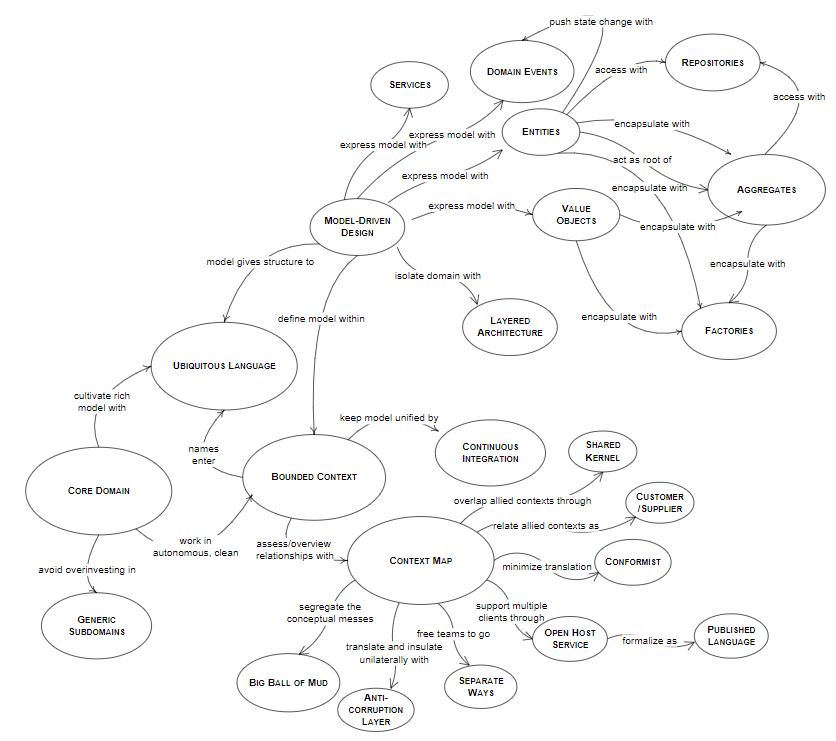
\includegraphics[height=0.5\textheight]{./part/Proyecto_ejecutivo/memoria_descriptiva/infoPreviaAntecedentes/img/DomainDrivenDesignReference}
    \caption{DomainDrivenDesignReference\cite{EricEvans2003DDTC}}\label{fig:DomainDrivenDesignReference}
\end{figure}

De todo este diagrama los conceptos en los que nos vamos a centrar son en los que surgen del componente "Model Driven Design" que son los elementos dentro de ese lenguaje que afectan al diseño del software a su nivel más elemental.

\begin{itemize}
    \item Entity: Elemento que contiene atributos definido por un identificador
    \item \textit{Value Object}: Elemento que tiene atributos pero no identificador
    \item Domain Event: Elemento que define una suceso inducido por la interacción entre los componentes del dominio.
    \item Aggregate: Cluster de elementos tratado como una unidad. Las referencias o acciones externas sobre sus elementos siempre se hacen a través de un único elemento de este cluster conocido como \textit{Agreggate Root}. Tiene reglas definidas de consistencia dentro de su delimitación.
    \item Repository: Es un mecanismo de interaccion para encapsular el acceso a tecnologías, como el almacenamiento en base de datos, para interactuar con ellas. La implementación no concierne al dominio.
    \item Service: Es una funcionalidad de interacción entre elementos de dominio. Encapsula lógica compleja que garantiza un comportamiento consistente.
\end{itemize}

Esta paradigma de diseño compone el elemento central en el paradigma de la arquitectura de capas o \gls{LayerArchitecture}. Se aisla esos contextos que definen nuestro dominio de implementaciones concretas ya sea para acceder al mismo o a las que accede el dominio. Por ejemplo, aislarlo de que se ejecute un servicio mediante una consola de comandos o desde una llamada http y que se guarde en una base de datos la información o se guarde en un archivo.

\paragraph{Hexagonal Architecture}

Dentro de las arquitecturas de capas vamos a utilizar un diseño de puerto y adaptadores o más conocido como \gls{HexagonalArchitecture}. El diagrama básico más utilizado en la teoría para representarlo se muestra en la figura~\cref{fig:hexagonalDiagram}. Como apreciación personal no le encuentro una utilidad real a este tipo de diagramas. El pretendido enfoque didáctico se pierde ya que el hexágono es una simple licencia estética. En el caso de existir más puertos de salida y entrada que los representados, el hexágono pierde todo el sentido. Cuando se enfrenta por primera vez este diagrama se tiende a intentar descifrar el sentído oculto detrás de la elección de la forma poligonal, no existe.

\begin{figure}[H]
    \centering
    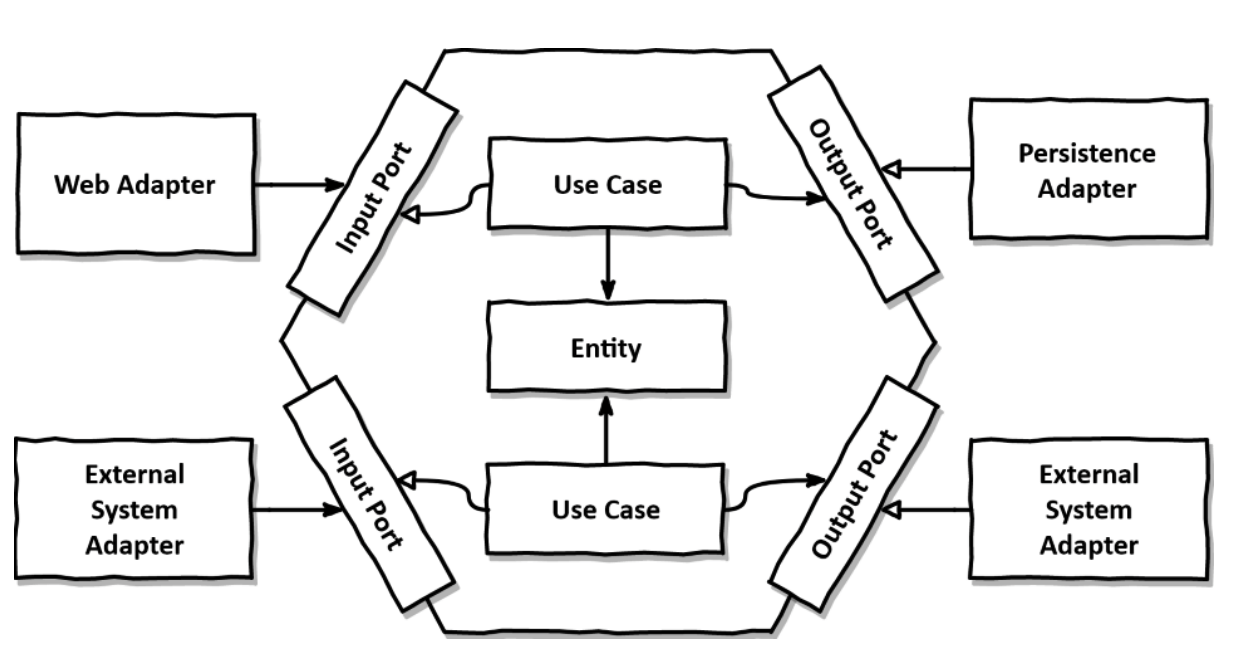
\includegraphics[height=0.3\textheight]{./part/Ejecucion/Seguimiento/CreateTaskUseCase/img/HexagonalDiagram}
    \caption{Hexagonal architecture diagram\cite{TomHombergs2019GYHD}}\label{fig:hexagonalDiagram}
\end{figure}

En este diagrama, el dominio está representado por una única entidad, o Entity, que se encuentra aislada de todo y no depende de ningún elemento. La aplicación está respresentada por los casos de uso, o UseCase, y utiliza el dominio dependiendo de él. La aplicación se aisla del exterior, la infraestructura, obligando a utilizar sus interfaces a los elementos que acceden, esto está representado por la flecha con cabeza hueca o de color blanco. y utilizando interfaces que será responsabilidad de la infraestructura implementar, desconociendo la aplicación su implementación particular.

En el diagrama~\cref{fig:layers} podemos ver este concepto más simplificado. El objetivo es expresar que la dependencia de las capas, expresada por las flechas, sea siempre de fuera hacia adentro. Queremos preservar del cambio el interior y exponer al cambio el exterior. Separar lo propenso al cambio de lo que no. Separar el UL de los detalles de implementación, que tienen su propio lenguaje.

\begin{figure}[H]
    \centering
    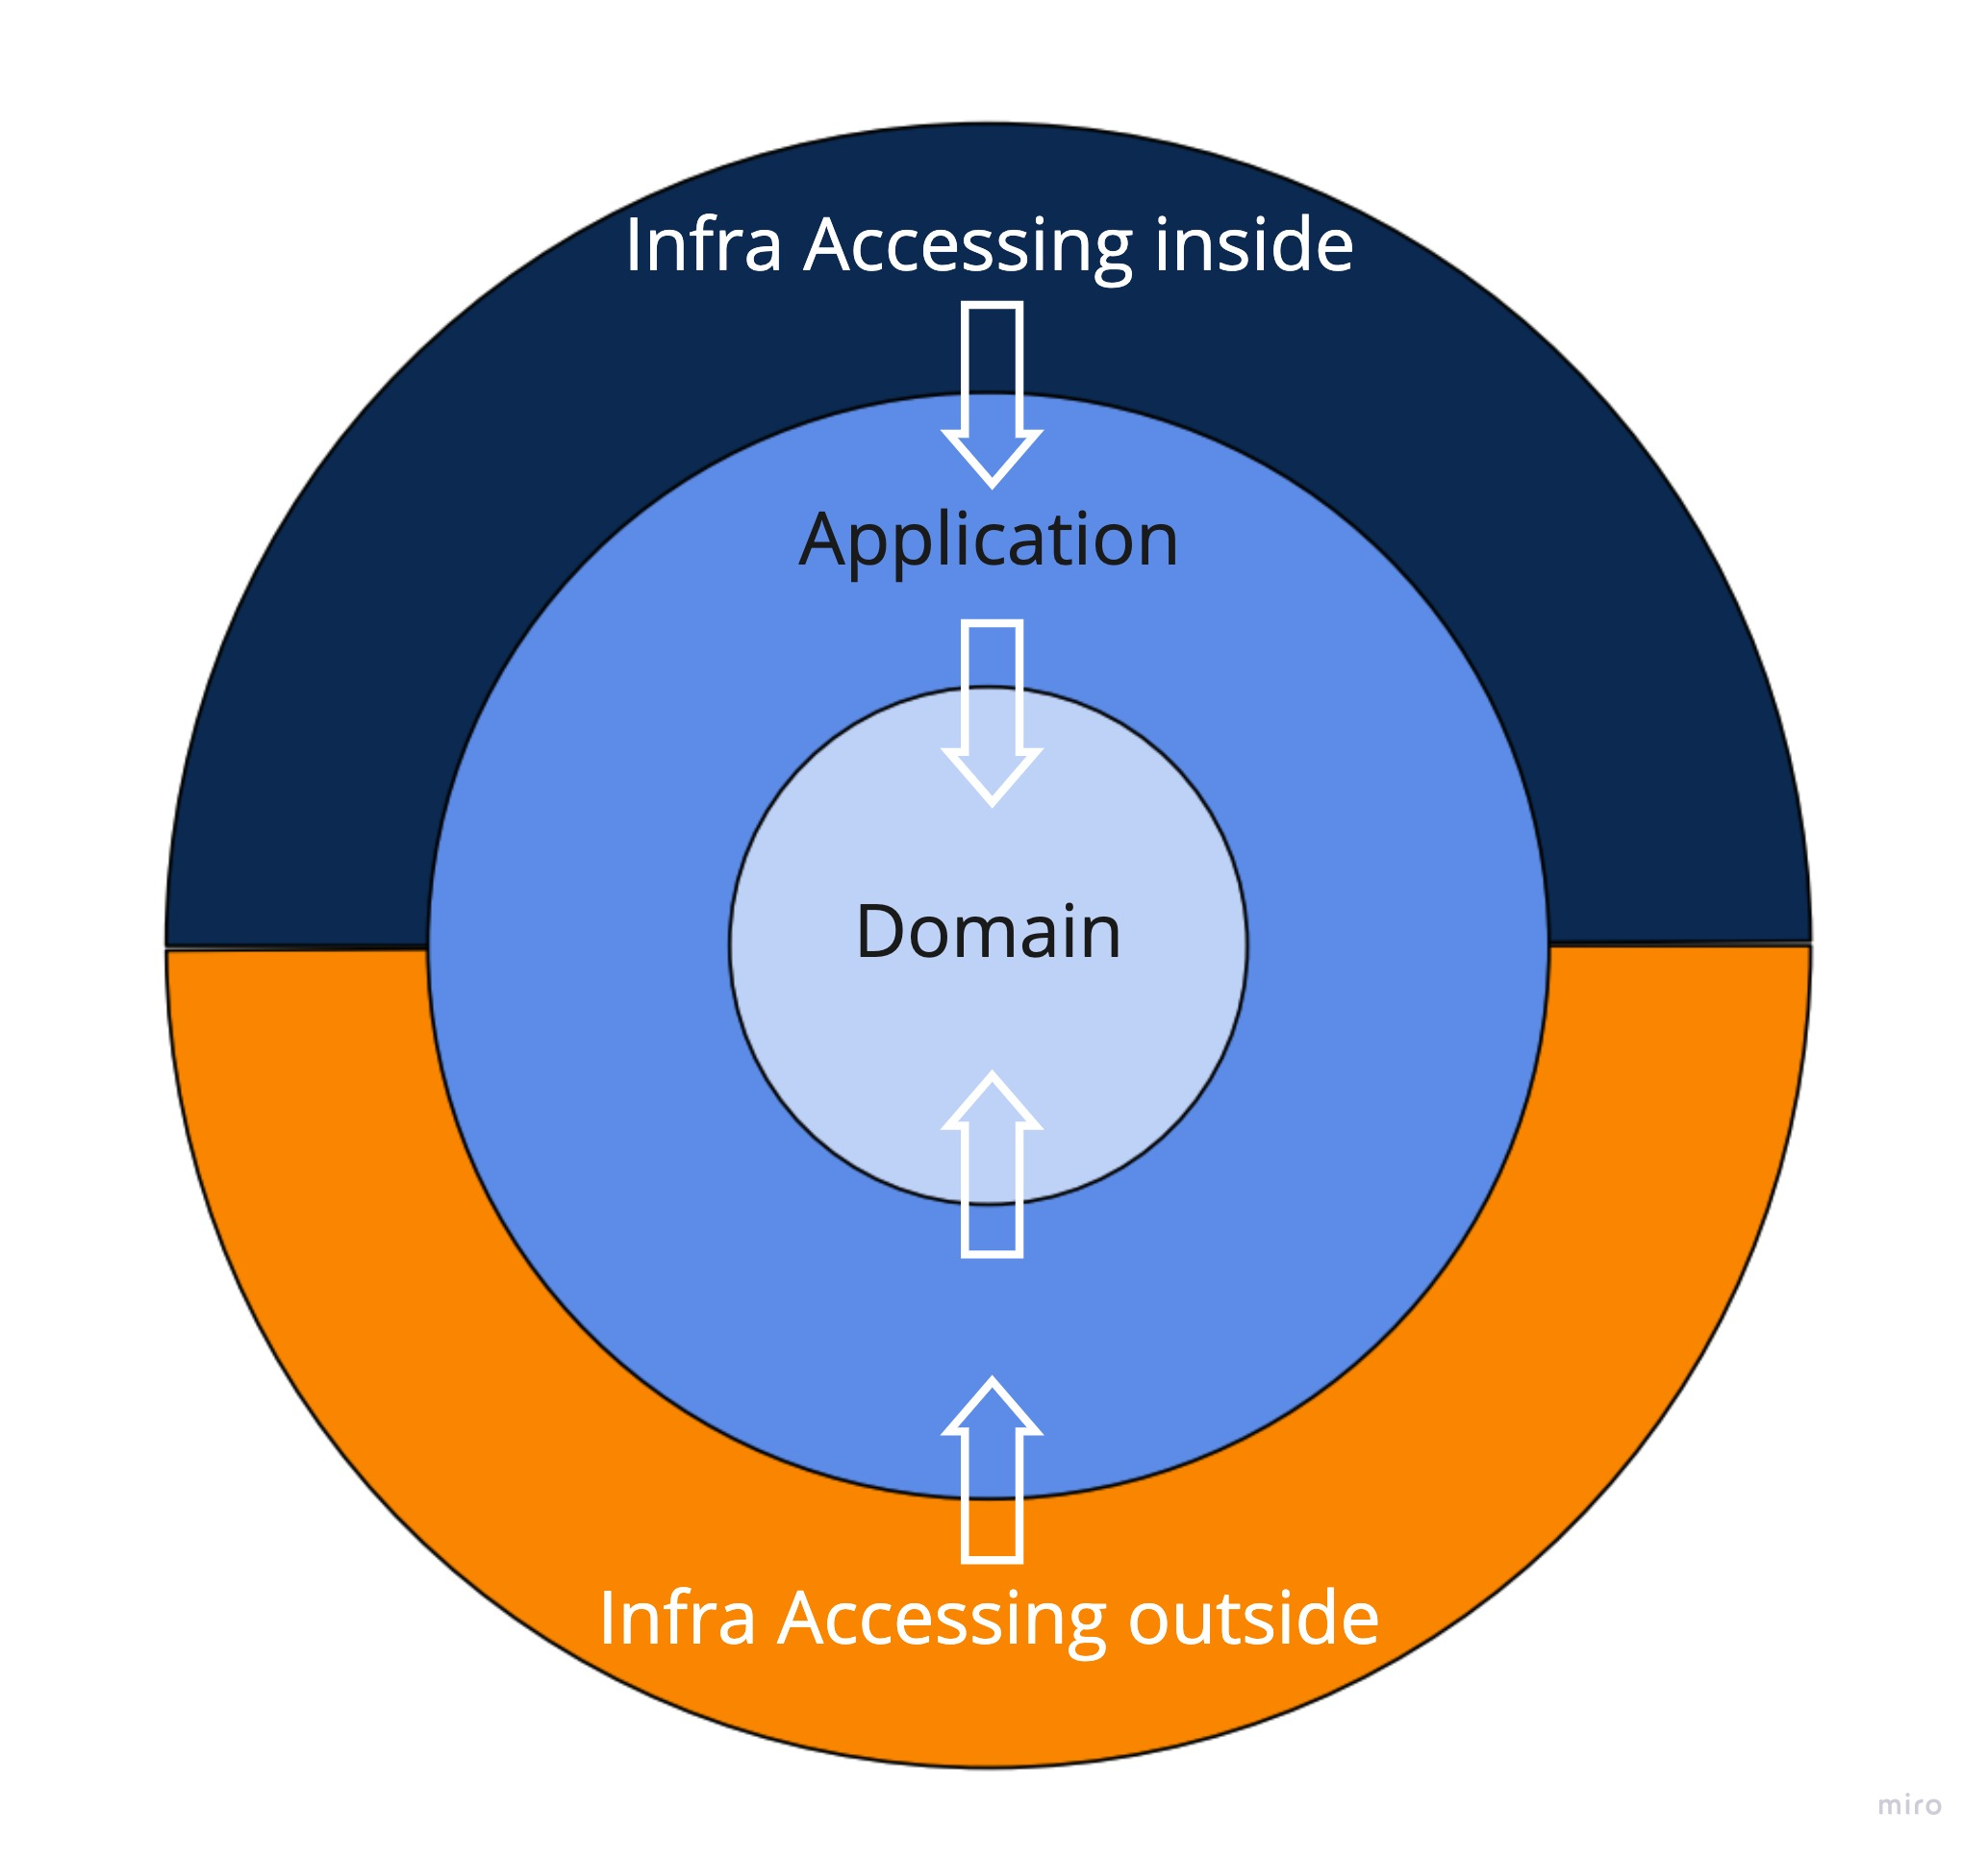
\includegraphics[height=0.3\textheight]{./part/Proyecto_ejecutivo/memoria_descriptiva/infoPreviaAntecedentes/img/PFM - Layer}
    \caption{Arquitectura de capas}\label{fig:layers}
\end{figure}

\paragraph{CQRS}

Junto con el concepto de arquitectura hexagonal y el\textit{DDD} vamos a aplicar el paradigma de diseño conocido como \gls{CQRS} (Command Query Responsibility Segregation). Es una técnica de diseño de arquitectura de software que separa la lógica de escritura (comandos) de la lógica de lectura (consultas) en sistemas de información. La idea es que las operaciones de escritura (comandos) y las operaciones de lectura (consultas) se manejen por separado, ya que tienen necesidades y características distintas. Mientras que las operaciones de escritura son responsables de modificar el estado de la aplicación, las operaciones de lectura son responsables de devolver información sobre ese estado sin modificarlo. Al separar estas dos responsabilidades, se pueden optimizar las operaciones de lectura para que sean más rápidas y escalables. Además, se puede diseñar una arquitectura de software más flexible, permitiendo una mayor adaptabilidad y evolución del sistema a medida que cambian los requisitos de la aplicación.

El resumen hasta ahora es que el diseño sigue una arquitectura hexagonal, con un enfoque\textit{DDD} en el dominio y un enfoque CQRS en los casos de uso. Es decir se diseñará un dominio rico y con un UL y se accederá a su funcionalidad a través de casos de uso que sigan el criterio de ser comandos y consultas.

\paragraph{Mapping}

El último detalle a explicar es cómo garantizar la separación efectiva de las capas en su uso de los elementos básicos con los que interactuan. Si un elemento de Infraestructura utiliza directamente una Entity de Dominio estaría saltando la capa de aplicación en su diagrama de dependencia. Bien es cierto que se mantendría la dependencia de fuera hacia adentro, pero se ha de tomar una decisión de hasta qué punto se quiere desacoplar una capa de otra. A esta decisión de diseño se le conoce como Estrategia de Mapping entre capas. Estrictamente cada capa requiere sus objetos de trabajo para estar desacoplada de las demás, pero como en todo aspecto de diseño está sometido a discusión acerca de seguir la teoría al pié de la letra y el pragmatismo de no verse envuelto en redundancias y sobredimensionar las soluciones.

En un extracto del libro Get Your Hands Dirty on Clean Architecture\cite{TomHombergs2019GYHD} podemos leer un extracto que es interesante rescatar ya que representa una conversación demasiado habitual entre compañeros de trabajo:

\textit{ The argument might have gone something like this:}

\begin{itemize}
    \item \textit{Pro-Mapping Developer:}
    \subitem  \textit{ If we don’t map between layers, we have to use the same model in both layers which means that the layers will be tightly coupled!}
    \item \textit{Contra-Mapping Developer:}
    \subitem \textit{ But if we do map between layers, we produce a lot of boilerplate code which is overkill for many use cases, since they’re only doing CRUD and have the same model across layers anyways!}
\end{itemize}
\textit{As is often the case in discussions like this, there’s truth to both sides of the argument. Let’s discuss some mapping strategies with their pros and cons and see if we can help those developers make a decision.}

Hay tantas estrategias como atajos dentro de este paradigma queramos asumir. Todo buen diseñador técnico debe saber tanto la teoría como los atajos que se pueden tomar. Evaluar los beneficios e inconvenientes y tomar una decisión con la que se ha de ser consecuente, y más importante en desarrollo, consistente. Esto quiere decir que una vez tomada una decisión debe ser una decisión en equipo que todos sigan. Es más eficiente un diseño imperfecto que sea consistente que un diseño perfecto en unos puntos e imperfecto en otros. Esto lleva al desorden a la hora de escribir código y complica la entrada de nuevos compañeros, el entendimiento del código existente con todas las consecuencias negativas que esto conlleva.

Los tipos de mapping que se documentan en este libro\cite{TomHombergs2019GYHD}:
\begin{itemize}
    \item The No Mapping Strategy~\cref{fig:nomapping}
    \item The Two-Way Mapping Strategy~\cref{fig:twowaymapping}
    \item The Full Mapping Strategy~\cref{fig:fullmapping}
    \item The One-Way Mapping Strategy~\cref{fig:onWaymapping}
\end{itemize}

Vamos a tomar diagramas del libro para entender cada estrategia. En todos los casos vemos simplificado el dominio a una única entidad, Account, y vemos como separa dicho dominio del acceso al caso de uso que envía dinero a una cuenta y del acceso a la infraestructura que guarda la información del envío de ese dinero.

\begin{figure}[H]
    \centering
    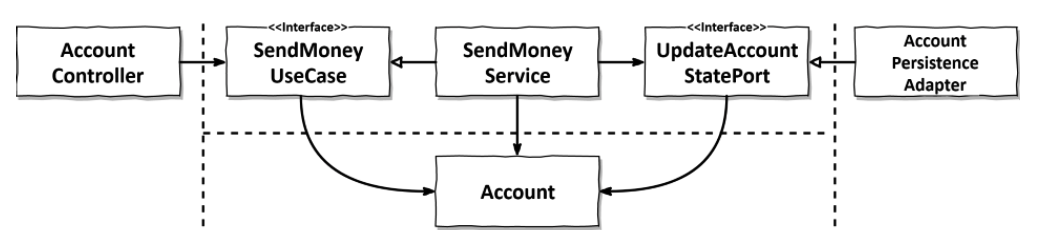
\includegraphics[height=0.1\textheight]{./part/Ejecucion/Seguimiento/CreateTaskUseCase/img/nomapping}
    \caption{No mapping strategy~\cite{TomHombergs2019GYHD}}\label{fig:nomapping}
\end{figure}

En la estrategia de No Mapping podemos ver en la figura~\cref{fig:nomapping} que tanto aplicación como Infraestructura dependen de Dominio. Esto evita todo código redundante, los \gls{DTO} (Data Transfer Object), pero resta flexibilidad. Si por detalles técnicos de una infraestructura concreta se requiere más o menos parámetros que los definidos en el Dominio o se deben guardar en otro formato que los definidos en Dominio enfrentaremos un problema.

\begin{figure}[H]
    \centering
    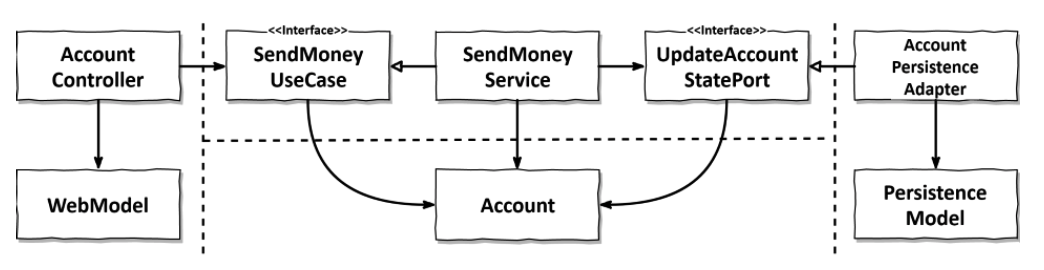
\includegraphics[height=0.1\textheight]{./part/Ejecucion/Seguimiento/CreateTaskUseCase/img/twowaymapping}
    \caption{Two way mapping strategy~\cite{TomHombergs2019GYHD}}\label{fig:twowaymapping}
\end{figure}

En la estrategia de Two-Way Mapping Strategy~\cref{fig:twowaymapping} nos deshacemos de este problema y creamos un modelo DTO que sirva para transportar la información de una capa a otra necesaria para conformar la Entidad. De esta forma puede evolucionar por separado. Seguimos contemplando ese posible problema problema entre la Aplicación, los casos de uso, y el Dominio. Además tenemos que escribir más código para crear las entidades a través de los DTO y viceversa.

\begin{figure}[H]
    \centering
    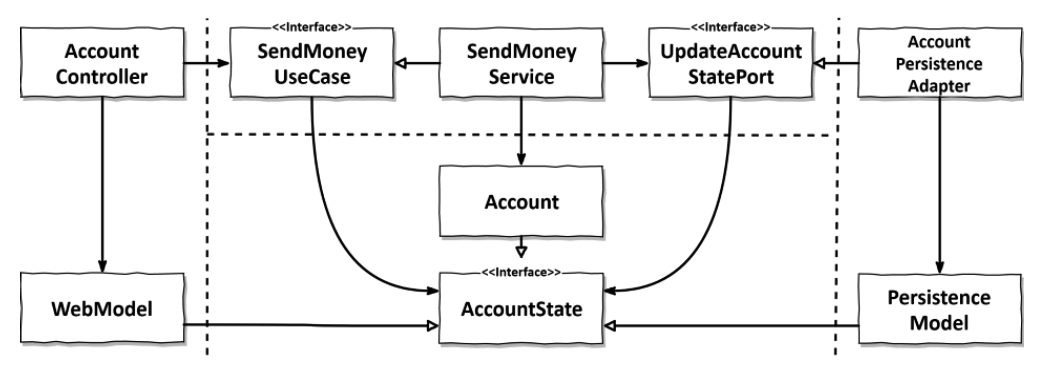
\includegraphics[height=0.1\textheight]{./part/Ejecucion/Seguimiento/CreateTaskUseCase/img/onWaymapping}
    \caption{One way mapping strategy~\cite{TomHombergs2019GYHD}}\label{fig:onWaymapping}
\end{figure}

En la figura de The One-Way Mapping Strategy~\cref{fig:onWaymapping} vemos que creamos una interfaz para la Entidad y hacemos depender de nuevo todas las capas de dicha interfaz. Se encuentran las capas más separadas y preparadas para el caso en el que se enfrente la necesidad de tener que crear distintas implementaciones aunque no se creen en un primer momento.

\begin{figure}[H]
    \centering
    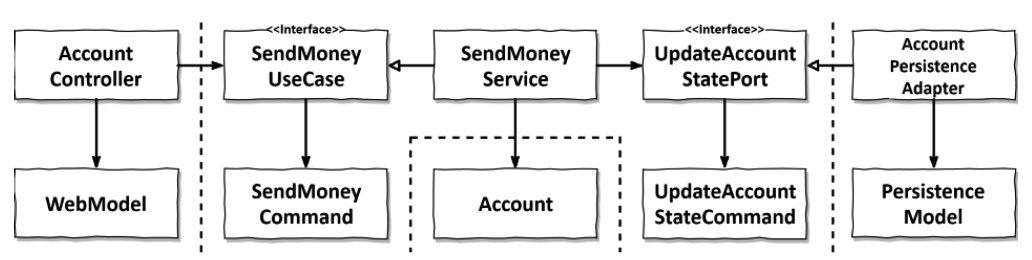
\includegraphics[height=0.1\textheight]{./part/Ejecucion/Seguimiento/CreateTaskUseCase/img/fullmapping}
    \caption{Full mapping strategy~\cite{TomHombergs2019GYHD}}\label{fig:fullmapping}
\end{figure}

En la figura de The Full Mapping Strategy~\cref{fig:twowaymapping} se opta por crear DTOs entre todas las capas. Es la solución más pura, pero el tradeoff es evidente: la cantidad de código a realizar es considerable y tiene que estar justificada con una necesidad de aislar hasta este punto.

No hay una regla de oro para elegir una estratégia que valga para todos los casos. Se reitera que debe ser una decisión de equipo, seguir la decisión todos y reevaluar con cada inconveniente que enfrente la decisión si se tiene que cambiar la estrategia.

Se puede ver el primer ejemplo en el un proyecto de ejecución que intentara resolver todas las decisiones y describir al detalle la solución a desarrollar no aportaría valor. Tomar una decisión de este tipo y documentarla, carece de utilidad porque no disponemos de información suficiente para tomar la decisión. Cuando nos enfrentamos al código es cuando podemos ver qué estrategia encaja mejor en nuestro caso.

\paragraph{Testing}
    Para el caso de uso de Create task siguiendo\ref{par:testing}

Primero tenemos que localizar los factores o variables independientes

\begin{itemize}
    \item Host
    \item Port
    \item CommunicationMode
    \item ExecutionMode
    \item Steps
\end{itemize}

luego las clases de equivalencia:

\begin{itemize}
    \item Host: valid/invalid
    \item Port: valid/invalid
    \item CommunicationMode: valid/invalid
    \item ExecutionMode: valid/invalid
    \item Steps: valid/invalid
\end{itemize}

Cabe reseñar que el trabajo de buscar las clases de equivalencia no es trivial. por ejemplo, en el caso de steps que es un array podría haberse pensado que se necesita probar con varios elementos en el array, validos e invalidos, pero no tiene sentido porque la lógica debe contemplar únicamente

o por ejemplo en el caso de Host o Port que tiene validaciones. podría pensarse que debería ponerse a prueba con varios casos que den invalido, al ser un string libre y que ponga a prueba dicha validación, pero estamos en el caso de uso, eso será responsabilidad del test unitario de Host y Port. para la lógica que nos atañe en este test lo único que importa es qué sucedera en el caso que sea válido o invalido.

En un ejemplo tan trivial puede llevar a subestimar el ejercicio de entender el alcance de la prueba y la correcta selección de las clases de equivalencia, pero es de suma importancia.

Bien pues con estas clases de equivalencia las posibilidades son \[ 2^5 = 32 \] casos con el método de pares se reduce a 6 y los pares posibles son 41

las combinaciones posibles son:

\begin{table}[H]
    \small
    \begin{tabular}{cccccc}
        \textbf{}   & \textbf{host} & \textbf{port} & \textbf{communicationMode} & \textbf{executionMode} & \textbf{sentences} \\
        \textbf{1}  & valid         & valid         & valid                      & valid                  & valid              \\
        \textbf{2}  & valid         & valid         & valid                      & valid                  & invalid            \\
        \textbf{3}  & valid         & valid         & valid                      & invalid                & valid              \\
        \textbf{4}  & valid         & valid         & valid                      & invalid                & invalid            \\
        \textbf{5}  & valid         & valid         & invalid                    & valid                  & valid              \\
        \textbf{6}  & valid         & valid         & invalid                    & valid                  & invalid            \\
        \textbf{7}  & valid         & valid         & invalid                    & invalid                & valid              \\
        \textbf{8}  & valid         & valid         & invalid                    & invalid                & invalid            \\
        \textbf{9}  & valid         & invalid       & valid                      & valid                  & valid              \\
        \textbf{10} & valid         & invalid       & valid                      & valid                  & invalid            \\
        \textbf{11} & valid         & invalid       & valid                      & invalid                & valid              \\
        \textbf{12} & valid         & invalid       & valid                      & invalid                & invalid            \\
        \textbf{13} & valid         & invalid       & invalid                    & valid                  & valid              \\
        \textbf{14} & valid         & invalid       & invalid                    & valid                  & invalid            \\
        \textbf{15} & valid         & invalid       & invalid                    & invalid                & valid              \\
        \textbf{16} & valid         & invalid       & invalid                    & invalid                & invalid            \\
        \textbf{17} & invalid       & valid         & valid                      & valid                  & valid              \\
        \textbf{18} & invalid       & valid         & valid                      & valid                  & invalid            \\
        \textbf{19} & invalid       & valid         & valid                      & invalid                & valid              \\
        \textbf{20} & invalid       & valid         & valid                      & invalid                & invalid            \\
        \textbf{21} & invalid       & valid         & invalid                    & valid                  & valid              \\
        \textbf{22} & invalid       & valid         & invalid                    & valid                  & invalid            \\
        \textbf{23} & invalid       & valid         & invalid                    & invalid                & valid              \\
        \textbf{24} & invalid       & valid         & invalid                    & invalid                & invalid            \\
        \textbf{25} & invalid       & invalid       & valid                      & valid                  & valid              \\
        \textbf{26} & invalid       & invalid       & valid                      & valid                  & invalid            \\
        \textbf{27} & invalid       & invalid       & valid                      & invalid                & valid              \\
        \textbf{28} & invalid       & invalid       & valid                      & invalid                & invalid            \\
        \textbf{29} & invalid       & invalid       & invalid                    & valid                  & valid              \\
        \textbf{30} & invalid       & invalid       & invalid                    & valid                  & invalid            \\
        \textbf{31} & invalid       & invalid       & invalid                    & invalid                & valid              \\
        \textbf{32} & invalid       & invalid       & invalid                    & invalid                & invalid
    \end{tabular}
    \caption{tab:table2}\label{tab:table2}
\end{table}

y los pares son

\begin{table}[H]
    \small
    \begin{tabular}{llll}
        \textbf{var1}          & \textbf{var2}     & \textbf{value1} & \textbf{value2} \\
        \textbf{host}          & port              & valid           & valid           \\
        \textbf{host}          & port              & valid           & notValid        \\
        \textbf{host}          & port              & notValid        & valid           \\
        \textbf{host}          & port              & notValid        & notValid        \\
        \textbf{host}          & executionMode     & valid           & valid           \\
        \textbf{host}          & executionMode     & valid           & notValid        \\
        \textbf{host}          & executionMode     & notValid        & valid           \\
        \textbf{host}          & executionMode     & notValid        & notValid        \\
        \textbf{host}          & communicationMode & valid           & valid           \\
        \textbf{host}          & communicationMode & valid           & notValid        \\
        \textbf{host}          & communicationMode & notValid        & valid           \\
        \textbf{host}          & communicationMode & notValid        & notValid        \\
        \textbf{host}          & steps             & valid           & valid           \\
        \textbf{host}          & steps             & valid           & notValid        \\
        \textbf{host}          & steps             & notValid        & valid           \\
        \textbf{host}          & steps             & notValid        & notValid        \\
        \textbf{port}          & executionMode     & valid           & valid           \\
        \textbf{port}          & executionMode     & valid           & notValid        \\
        \textbf{port}          & executionMode     & notValid        & valid           \\
        \textbf{port}          & executionMode     & notValid        & notValid        \\
        \textbf{port}          & communicationMode & valid           & valid           \\
        \textbf{port}          & communicationMode & valid           & notValid        \\
        \textbf{port}          & communicationMode & notValid        & valid           \\
        \textbf{port}          & communicationMode & notValid        & notValid        \\
        \textbf{port}          & steps             & valid           & valid           \\
        \textbf{port}          & steps             & valid           & notValid        \\
        \textbf{port}          & steps             & notValid        & valid           \\
        \textbf{port}          & steps             & notValid        & notValid        \\
        \textbf{executionMode} & communicationMode & valid           & valid           \\
        \textbf{executionMode} & communicationMode & valid           & notValid        \\
        \textbf{executionMode} & communicationMode & notValid        & valid           \\
        \textbf{executionMode} & communicationMode & notValid        & notValid        \\
        executionMode          & steps             & valid           & valid           \\
        executionMode          & steps             & valid           & notValid        \\
        executionMode          & steps             & notValid        & valid           \\
        executionMode          & steps             & notValid        & notValid        \\
        communicationMode      & steps             & valid           & valid           \\
        communicationMode      & steps             & valid           & notValid        \\
        communicationMode      & steps             & notValid        & valid           \\
        communicationMode      & steps             & notValid        & notValid
    \end{tabular}
    \caption{tab:table3}\label{tab:table3}
\end{table}

El tests quedaría entonces como sale en la figura \ref{tab:createTaskPairWiseTest}

\begin{table}[H]
    \small
    \begin{tabular}{rllllll}
        case & host     & port     & ExeMode  & ComMode  & steps    & Expected Result        \\
        1    & valid    & valid    & valid    & valid    & valid    & OK                     \\
        2    & valid    & notValid & notValid & notValid & notValid & PortInvalidError       \\
        3    & notValid & valid    & notValid & valid    & notValid & HostInvalidError       \\
        4    & notValid & notValid & valid    & notValid & valid    & HostInvalidError       \\
        5    & ~valid   & valid    & valid    & notValid & notValid & CommunicationModeError \\
        6    & ~valid   & notValid & notValid & valid    & valid    & PortError
    \end{tabular}
    \caption{tab:createTaskPairWiseTest}\label{tab:createTaskPairWiseTest}
\end{table}

En la instaciación de una nueva Task tenemos los

Primero tenemos que localizar los factores o variables independientes

\begin{itemize}
    \item Number of steps
    \item execution Mode
    \item Communication Mode
\end{itemize}

luego las clases de equivalencia:

\begin{itemize}
    \item NSteps: 0,1,>2
    \item ExMod: Automatic, Manual
    \item ComMode: Server Stream,Client Stream, Bidirectional y Unary
\end{itemize}

tenemos entonces \[ 3*2*4 = 24 \] posibilidades pares obtenemos 27 al final queda reducidos a 13 casos. Vemos que la eficiencia en reducción de casos disminuye cuanto menos combinaciones hay. El diseño de los tests queda tal y como se ve en la tabla \ref{tab:taskTestPairwiseCases}

\begin{table}[H]
    \small
    \begin{tabular}{ccccl}
        \textbf{}   & \textbf{NSteps} & \textbf{ExeMod} & \textbf{ComMode} & \multicolumn{1}{c}{\textbf{Expected Result}}  \\
        \textbf{1}  & 0               & automatic       & serverStream     & NewTaskMustHaveAtLeastOneStepError            \\
        \textbf{2}  & 1               & automatic       & clientStream     & OK                                            \\
        \textbf{3}  & 1               & manual          & bidirectional    & OK                                            \\
        \textbf{4}  & 1               & automatic       & unary            & OK                                            \\
        \textbf{5}  & 1               & manual          & serverStream     & OK                                            \\
        \textbf{6}  & \textgreater{}2 & manual          & unary            & CommunicationModeCanOnlyHaveOneStepError      \\
        \textbf{7}  & \textgreater{}2 & automatic       & serverStream     & CommunicationModeCanOnlyHaveOneStepError      \\
        \textbf{8}  & \textgreater{}2 & manual          & clientStream     & OK                                            \\
        \textbf{9}  & \textgreater{}2 & automatic       & bidirectional    & ManualBidirectionalTaskOnlyCanHave2StepsError \\
        \textbf{10} & 0               & automatic       & clientStream     & TaskMustHaveAtLeastOneStepError               \\
        \textbf{11} & 0               & manual          & bidirectional    & TaskMustHaveAtLeastOneStepError               \\
        \textbf{12} & 0               & automatic       & unary            & TaskMustHaveAtLeastOneStepError               \\
        \textbf{13} & 0               & manual          & serverStream     & TaskMustHaveAtLeastOneStepError
    \end{tabular}
    \caption{tab:taskTestPairwiseCases}\label{tab:taskTestPairwiseCases}
\end{table}

Ahora vamos a ver cómo la arquitectura protege la calidad del sistema de las implementaciones en proceso de investigación. Sabemos que el looper tiene los siguientes factores:

\begin{figure}[H]
    \centering
    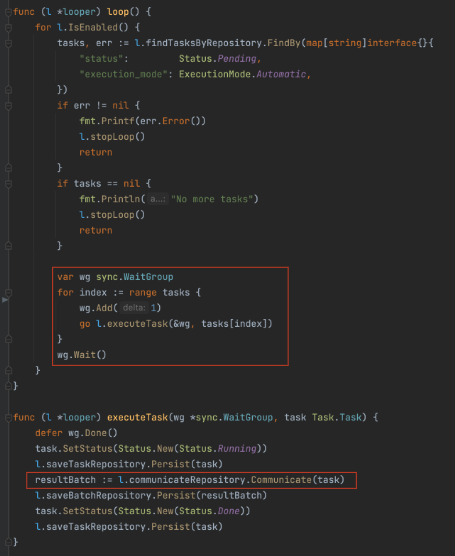
\includegraphics[height=0.3\textheight]{./part/Ejecucion/Seguimiento/Testing/img/Looper}
    \caption{testing looper.go detail}\label{fig:testingLooper}
\end{figure}

el punto clave de la figura \ref{fig:testingLooper} señalado en el recuadro rojo es el adaptador de comunicación GRPC es un adaptador experimental que debido a la inexperiencia en su uso está desarrollado de forma ineficiente. Hemos extraido toda la lógica posible a este servicio que es la parte core:

El adaptador puede tener múltiples errores inesperados, no conseguir comunicar con el servicio cliente, timeouts, malas implementaciones de la librería, pero se ha protegido al dominio de todo esto mediante una interfaz que garantiza que ante cualquier error se devuelve siempre un resultado. Lo único que quedaría por implementar y testear sería que el proceso no consiguiera terminar y se quedara la gorutine en un proceso infinito. para ello en el proceso de descubrimiento del lenguaje sabemos que hay un punto débil en el dominio. No hemos hehco uso de una herramienta de Golang que se conoce como context. que permite gestionar los timeouts de las gorutines evitando que que queden procesos hijos sin control.

Tengamos en cuenta que hemos extraido de toda la comunicación con el cliente una interfaz útil y única para comunicarnos, una lógica de negocio que entender en pocas lineas de código y explicar su funcionamiento, controlarlo y testearlo y aún así encontramos puntos débiles que mejorar en ese diseño. Si a esto le hubieramos sumado las lineas de codigo que hay detrás de la interfaz de comunicacion sería ingestionable. para cuantificar esto vamos a hacer una aproximación al diseño del test necesario para cubrir el adaptador de comunicacion

El código completo se encuentra en el repositorio github. Simplificando para esta explicación el pseudocódigo sería el siguiente

\begin{verbatim}
connection, err := grpc.Dial()
    serverStream:
        client.CallServerStream(request)
        responseStream.Recv()
    Bidirectional:
        client.CallBidirectional()
        async stream.Recv()
        async stream.Send()
        stream.CloseSend()
    ClientStream:
        client.CallClientStream()
        stream.Send
        stream.CloseAndRecv()
    Unary
        client.CallUnary()
connection.Close()
\end{verbatim}

vemos que hay mucha lógica junta, múltiples responsabilidades y por lo tanto no es un buen diseño. Como se demuestra mejor es intentando diseñar los tests. Para empezar extraer del código estas clases de equivalencia y factores no ha sido sencillo ya que hay multiples gestiones de errores dispersos por el código y es un código extenso 178 lineas. Esto ocurre en multitud de ocasiones, ya sea debido al tiempo, desconocimiento o mala praxis nos encontramos con códigos de esta magnitud. La arquitectura y todo este proceso lo que hace es protegernos de estas secciones sucias.

factores y posibles respuestas:

\begin{itemize}
    \item grpc.Dial(): err, connection
    \item client.CallServerStream(request): err,stream
    \item responseStream.Recv(): EOF,err,nil
    \item client.CallBidirectional(): error,stream
    \item stream.Recv(): EOF,err, result
    \item stream.Send(): EOF, nil,err
    \item stream.CloseSend() err,nil
    \item client.CallClientStream(): err, stream
    \item stream.Send: err, nil
    \item stream.CloseAndRecv(): err, nil
    \item client.CallUnary(): err,nil
    \item connection.Close(): err, nil
\end{itemize}

Si no entendieramos bien el concepto de clase de equivalencia podría llevarnos a un mal diseño de los tests o a hacerlo más complejo. Aunque hay factores que tiene tres respuestas posibles EOF y nil tienen que ir de la mano, significa que no ha habido error, primero obtienes un nil en el error y luego obtienes un error tipo EOF que significa que todo ha terminado correctamente. y luego tenemos cuando obtenmos un error distinto de EOF, si esto ocurre nos importa cuaántas veces haya ocurrido el caso sin error, será error igualmente. Con lo cual las clases de equivalencia serían

\begin{itemize}
    \item grpc.Dial(): err, connection
    \item client.CallServerStream(): err,stream
    \item responseStream.Recv(): nil\&EOF,err
    \item client.CallBidirectional(): error,stream
    \item stream.Recv(): nil\&EOF,err
    \item stream.Send(): nil\&EOF,err
    \item stream.CloseSend() err,nil
    \item client.CallClientStream(): err, stream
    \item stream.Send: err, nil
    \item stream.CloseAndRecv(): err, nil
    \item client.CallUnary(): err,nil
    \item connection.Close(): err, nil
\end{itemize}

para este caso tendríamos \[ 2^{12} = 4096 \] combinaciones posibles que pairwise reduce a 59 tests. aquí se ve la potencia del método. Volviendo posible un testing con ciertas garantías incluso en un código como el que nos ocupa.


\paragraph{Docker}

Docker es el sistema de gestión de contenedores más utilizado en la industria a día de hoy. Según la misma página oficial de Docker un contendor se define como: "A container is a standard unit of software that packages up code and all its dependencies so the application runs quickly and reliably from one computing environment to another. A Docker container image is a lightweight, standalone, executable package of software that includes everything needed to run an application: code, runtime, system tools, system libraries and settings."~\cite{docker}

El sistema se basa en la definición de imágenes que no son más que las instrucciones para la construcción de esos contenedores mediante el sistema de Docker Engine. Difieren de las máquinas virtuales tal y como se muestra en la comparativa~\cref{fig:Docker vs VM}.

Esto permite correr multiples aplicaciones con multiples requerimientos en cualquier máquina sin tener que instalar dichas dependencias de forma local, evitando incompatibilidades e interacciones no deseadas. Permite ofrecer entregables consistentes a los clientes de forma que el software y todo aquello que necesita para ejecutarse se entregan de forma conjunta, evitando problemas de instalación.

\begin{figure}[H]
    \centering
    \includegraphics[height=0.3\textheight]{./part/Proyecto_ejecutivo/memoria_descriptiva/prestaciones/docker/img/dockerVsVM}
    \caption{Docker vs VM.\cite{docker}}\label{fig:Docker vs VM}
\end{figure}

Las claves de Docker se basan en:
\begin{itemize}
    \item permite trabajar en el desarrollo de distintos proyectos con distintos requerimientos en una misma máquina sin la complejidad de mantener las dependencias de cada proyecto. O trasladarse a otra máquina y seguir trabajando de forma rápida al no tener que ponerse a instalar dichas dependencias de nuevo
    \item permite trabajar en equipo ya que cada cambio en las dependencias queda expresado en los cambios que se realizan de las imagenes de los contenedores que están disponibles para todo el equipo
    \item permite configurar el sistema para desarrollar o para producción de forma consistente con sus distintas diferencias en las dependencias necesarias, evitando problemas en el cambio de entorno de desarrollo y producción
\end{itemize}
\subsubsection{Descripción del proyecto}
    
\begin{figure}[H]
    \centering
    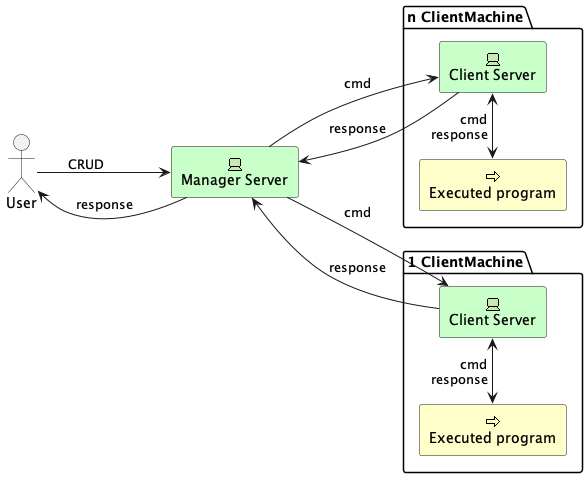
\includegraphics[height=0.4\textheight]{part/memoria_descriptiva/systemConcept}
    \caption[]{}\label{fig:systemConcept}
\end{figure}

Los componentes de esta solucion seran:
\begin{itemize}
    \item el manager server que guardará las tareas, las ejecutará y guardará el resultado.
    \item el client server que recepcionará las llamadas del manager con el comando y las ejecutará en el servidor cliente devolviendo los resultados al manager
    \item el programa a ejecutar. En nuestro caso haremos pruebas con varios ejecutables básicos, pero habrá un programa de control PID par aun motor de corriente continua
\end{itemize}

Se puede ver un diagrama conceptual del sistema en la figura~\ref{fig:systemConcept}. Vamos a proceder a describir cada uno de los programas de forma detallada. Esta descripción estará compuesta de los siguientes elementos:

\begin{itemize}
    \item diagrama de los componentes con los elementos con los que interacciona
    \item diagrama de objetos de sus elementos de dominio
    \item casos de uso: descripción y diagrama
    \item diagramas de procesos
    \item estructura de carpeta para la organización del código
\end{itemize}

\paragraph{Manager Server}

\begin{figure}[H]
    \centering
    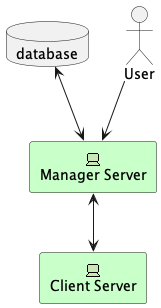
\includegraphics[height=0.4\textheight]{part/memoria_descriptiva/managerServerConcept}
    \caption[Diagrama componentes]{}\label{fig:managerServerConcept}
\end{figure}

\subparagraph{Dominio}

En el diagrama UML~\ref{fig:managerDomain} vemos que el dominio de Manager se compone de dos modulos: uno para las tareas y otro para los resultados. Vamos a ir explicando uno por uno:

\begin{itemize}
    \item Core
        \begin{itemize}
        \item Id todos los ids extenderan de este id, contiene un uuid, no sabemos que paquete usaremos para generarlos, es una de las pocas dependencias externas que vamos a tener dentro del dominio y queremo encapsularla lo máximo posible por si hubera que cambiarla. Además de esta forma los ids de las entities no se confunden en su tipo. si por ejemplo buscas una task mediante un id que corresponde a un result, si fueran del mismo tipo daría lugar a confusión porque no lo encontraríamos pero no nos advertiría de nuestro error
        \item Event todos los eventos del sistema extenderan del evento este
    \end{itemize}
    \item Task
        \begin{itemize}
        \item TaskId
        \item Host: es un Value Object compuesto por el valor del host, es un string pero el Value Object garantiza que es un valor válido, si no devuelve un error
        \item Port: es un Value Object compuesto por el valor del puerto, es un string pero el Value Object garantiza que es un valor válido, si no devuelve un error
        \item CommunicationMode: es un enum para expresar esa tarea de las formas de comunicación posibles que hay entre dos servidores cual sera la utilizada
            \begin{itemize}
                \item UNARY
                \item SERVER\_STREAM
                \item CLIENT\_STREAM
                \item BIDIRECTIONAL
            \end{itemize}
        \item ExecutionMode: es un enum
            \begin{itemize}
                \item MANUAL
                \item AUTOMATIC
            \end{itemize}
        \item Status: es un enum
            \begin{itemize}
                \item PENDING
                \item RUNNING
                \item SUCCESSFUL
                \item FAILED
            \end{itemize}
    \end{itemize}
    \item Step: cada tarea puede componerse en distintos pasos. Por ejemplo queremos poder poner en marcha el motor durante 15 segudos y luego llevarlo a una posición de inicio
    \begin{itemize}
      \item StepId
      \item sentence: será un string de contenido libre que el servidor cliente ejecutará en su sistema, dependerá de él tener instalado dicho programa y corroborar que la sintaxis es la correcta
    \end{itemize}
    \item TaskCreatedEvent. Cuando se cree una tarea se emitirá un evento, habrá un manejador de eventos que actuará en consecuencia. Si es una tarea automatizada y el loop de ejecución está parado lo pondrá en marcha.
    \item TaskModifiedEvent: si una tarea es modificada se emitirá un evento, habrá un manejador de eventos que actuará en consecuencia. Si la tarea vuelve a ser puesta a pending, es automatizada y el loop de ejecución está parado lo pondrá en marcha
    \item TaskDeletedEvent: si una tarea es modificada se emitirá un evento, habrá un manejador de eventos que actuará en consecuencia.
\end{itemize}

\begin{figure}[H]
    \centering
    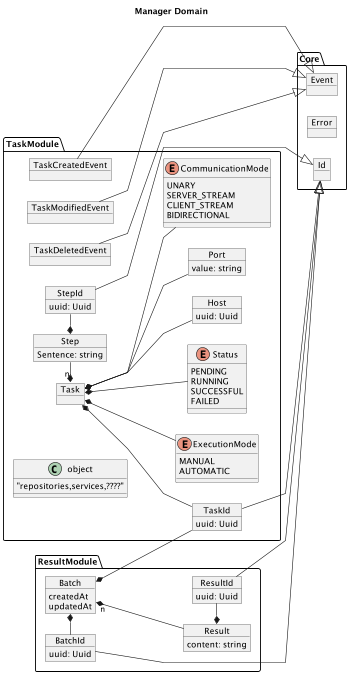
\includegraphics[height=0.4\textheight]{part/memoria_descriptiva/managerDomain}
    \caption[Diagrama de objetos de dominio]{}\label{fig:managerDomain}
\end{figure}



\subparagraph{casos de uso}

Vamos a describir los casos de uso que podrán ejecutarse en el programa manager

\textbf{crear tarea}

\begin{figure}[H]
    \centering
    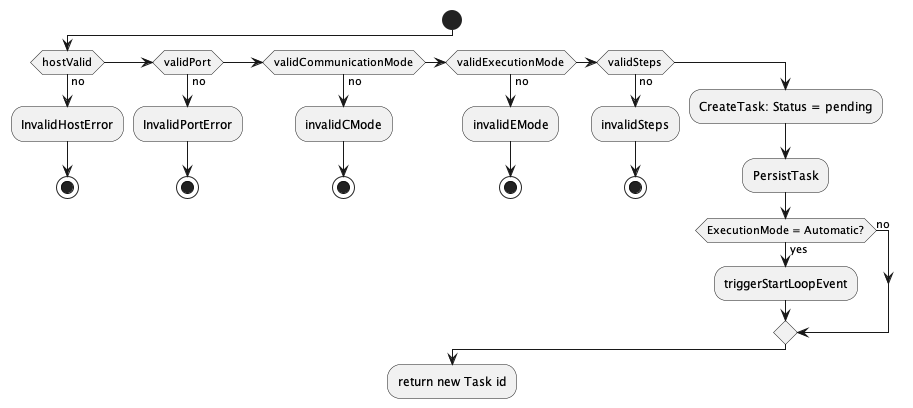
\includegraphics[height=0.3\textheight]{part/memoria_descriptiva/createTaskUseCase}
    \caption[Diagrama de objetos de dominio]{}\label{fig:createTaskUseCase}
\end{figure}

\textbf{obtener tarea}

\begin{figure}[H]
    \centering
    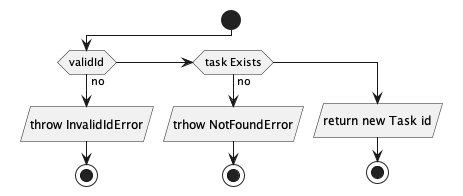
\includegraphics[height=0.3\textheight]{part/memoria_descriptiva/getTaskUseCase}
    \caption[Diagrama de objetos de dominio]{}\label{fig:getTaskUseCase}
\end{figure}

\textbf{listar tareas}

Uno de los puntos más amplios en una API CRUD es el filtrado de datos. No entra dentro del ámbito de este proyecto crear un sistema de filtrado que incluya la paginación. En este caso habría que crear una nomenclatura de filtros de cara al usuario y un sistema que los procese, devolviendo error ante un filtro erroneo o el listado de tareas que responda a dicho filtro. En nuestro caso devolveremos todas las tareas.

\textbf{actualizar tareas}

\begin{figure}[H]
    \centering
    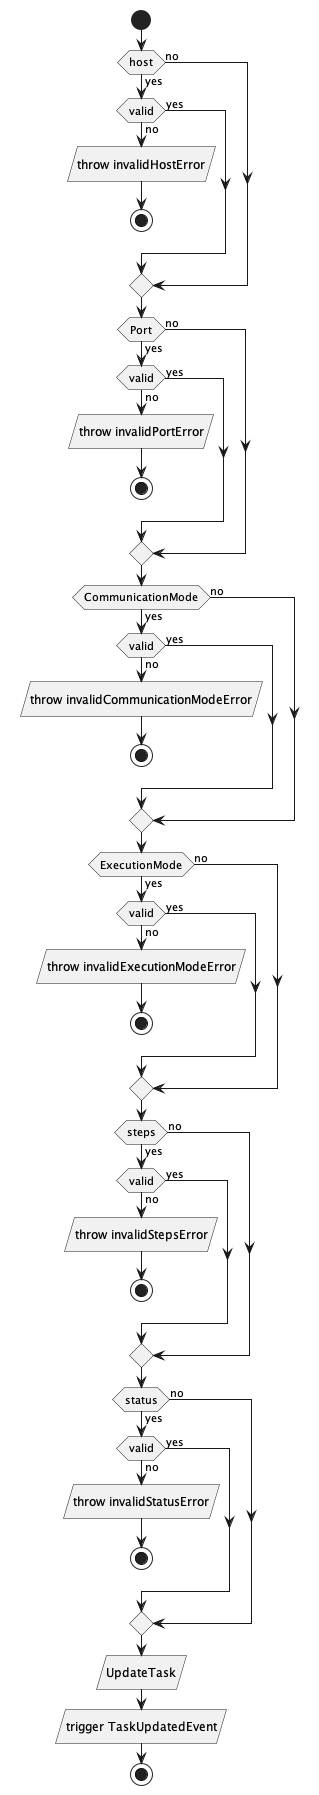
\includegraphics[height=0.5\textheight]{part/memoria_descriptiva/updateTaskUseCase}
    \caption[Diagrama de objetos de dominio]{}\label{fig:updateTaskUseCase}
\end{figure}

\textbf{eliminar tareas}

\begin{figure}[H]
    \centering
    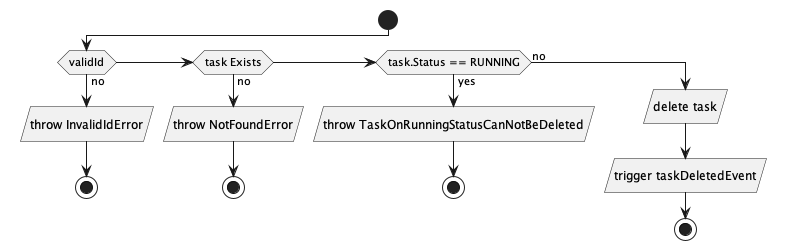
\includegraphics[height=0.2\textheight]{part/memoria_descriptiva/deleteTaskUseCase}
    \caption[Diagrama de objetos de dominio]{}\label{fig:deleteTaskUseCase}
\end{figure}

\subparagraph{estructura de carpetas}

Una de las partes mas importantes de un proyecto de software es que la estructura de carpetas hable sobre cómo está diseñado el software, sobre de qué va el software. qué es lo que hace y sobre que componentes interactua

En el proyecto constará de 4 carpetas principales
\dirtree{%
    .1 Project .
        .2 Adapter.
        .2 Application.
        .2 Domain.
        .2 Bootstrap.
}

Bootstrap será donde hagamos la composición de la aplicación, es decir la inyección de dependencias.

Vamos a desplegar la estructura capa por capa

\textbf{Adapters}

\dirtree{%
.1 Adapter.
    .2 in.
        .3 GRPC.
            .4 CreateEntityGrpcCall.
        .3 Console.
            .4 CreateEntityTerminalCommand.
    .2 out.
        .3 Email.
            .4 SendEmailOnCreationImplementation (*1).
        .3 Mysql.
            .4 SaveEntityImplementation (*2).
}

\textbf{Aplicación}

\dirtree{%
.1 Application.
    .2 Port.
        .3 in.
            .4 Entity.
                .5 CreateUseCase.
                    .6 CreateCommand.
                        .7 CreateCommand (using sendEmail param in this example).
                        .7 CreateUseCase.
                    .6 SomeEventHandler.
                        .7 CreationEvent.
                        .7 CreationEventUseCase.
        .3 out.
            .4 Email.
                .5 SendEmailConCreation (interface for *1).
}

\textbf{Dominio}

\dirtree{%
.1 Domain.
    .2 Core.
        .3 Id.
        .3 Event.
        .3 Error.
    .2 Task.
        .3 Id.
        .3 Task.
        .3 Host.
        .3 Port.
        .3 CommunicationMode.
        .3 ExecutionMode.
        .3 Status.
        .3 Step.
            .4 Id.
            .4 StepEntity.
            .4 StepVo.
            .4 Repository.
                .5 Find.
                .5 Save.
                .5 Search.
                .5 Delete.
                .5 Update.
            .4 Service.
                .5 Finder.
                .5 Creator.
                .5 Updater.
                .5 Eraser.
                .5 Searcher.
        .3 Repository.
            .4 Find.
            .4 Save.
            .4 Search.
            .4 Delete.
            .4 Update.
        .3 Service.
            .4 Finder.
            .4 Creator.
            .4 Updater.
            .4 Eraser.
            .4 Searcher.
    .2 Result.
}

Queda pendiente implementar aplicación e infraestructura. Cabe reseñar el apartado de aplicación loop handler. Vamos a detenernos en este concepto de aplicación que si merece la pena mención

\textbf{ejecutar loop de tareas automaticas}

handler que implementará aplicación porque el manual-automatic es muy complejo. al final habrá en este proceso muchos conceptos que descubriremos core de la aplicación y debieran ser dominio, pero como tenemos que descubrirlos vamos a implementarlos en aplicación haciendo uso de interfaces de infraestructura y de elementos de dominio. Si vemos claramente que algo puede convertirse en dominio lo introduciremos.


\paragraph{Client Server}

Hay que tener en cuenta que en este programa será casi todo infrestructura. ya que una vez recepcionado el comando mediante el RPC
solo quedará

En esta memoria descriptiva vamos a diseñar un sistema que tenga palabras clave para diferenciar un comando de pid y otro totalmente distinto. ya que si queremos ejecutar un simple comando de consola en el servidor cliente.

Las posibilidades son tantas como comandos haya instalados en el servidor cliente.

por ejemplo si el comando es ./runMyComand --arg=arg

como un típico comando de consola quedará a cargo del usuario de este progrmaa cliente implementar la interfaz

\paragraph{Control Program}

Casos de uso todas las funciones del engine y diseñarlo para que la infra sea a través de consola de comandos (preparando para que luego debido a la comunicación rpc devolver los datos sea muy complicado si lo dividimos en otro comando y decidimos absorver este dominio)

El sistema está pensado para que el programa a ejecutar sea de libre decisión del cliente. pero vamos a aprovechar la oportunidad para crear un programa de control y profundizar tanto en el uso del lenguaje como en los conocimientos relacionados con este master. En concreto el control automático. Uno do los programas que podrá ejecutar será un control PID.
\subsubsection{Prestaciones}
    \paragraph{Utilización}
    De cara al usuario cliente de este sistema dispondrá de:
    \begin{itemize}
        \item Un sistema para introducir y gestionar tareas para ejecutar en sistemas remotos de forma automática o manual
        \item Un programa cliente para ofrecer al público. Cualquier servidor con este programa instalado podrá recibir tareas desde el manager que se ejecutarán en su servidor de forma automática.
        \item Un programa de control pid para un microcontrolador para controlar un motor de corriente continua ejecutable desde consola. Por lo tanto cualquier cliente podrá instalarlo en su servidor y temporizar tareas sobre este programa.
    \end{itemize}

En un ejemplo básico de uso podríamos tener una puerta automática controlada por un microcontrolador y ejecutar la apertura desde el manager.

\paragraph{Seguridad y calidad}\label{par:testing}
    Para el caso de uso de Create task siguiendo\ref{par:testing}

Primero tenemos que localizar los factores o variables independientes

\begin{itemize}
    \item Host
    \item Port
    \item CommunicationMode
    \item ExecutionMode
    \item Steps
\end{itemize}

luego las clases de equivalencia:

\begin{itemize}
    \item Host: valid/invalid
    \item Port: valid/invalid
    \item CommunicationMode: valid/invalid
    \item ExecutionMode: valid/invalid
    \item Steps: valid/invalid
\end{itemize}

Cabe reseñar que el trabajo de buscar las clases de equivalencia no es trivial. por ejemplo, en el caso de steps que es un array podría haberse pensado que se necesita probar con varios elementos en el array, validos e invalidos, pero no tiene sentido porque la lógica debe contemplar únicamente

o por ejemplo en el caso de Host o Port que tiene validaciones. podría pensarse que debería ponerse a prueba con varios casos que den invalido, al ser un string libre y que ponga a prueba dicha validación, pero estamos en el caso de uso, eso será responsabilidad del test unitario de Host y Port. para la lógica que nos atañe en este test lo único que importa es qué sucedera en el caso que sea válido o invalido.

En un ejemplo tan trivial puede llevar a subestimar el ejercicio de entender el alcance de la prueba y la correcta selección de las clases de equivalencia, pero es de suma importancia.

Bien pues con estas clases de equivalencia las posibilidades son \[ 2^5 = 32 \] casos con el método de pares se reduce a 6 y los pares posibles son 41

las combinaciones posibles son:

\begin{table}[H]
    \small
    \begin{tabular}{cccccc}
        \textbf{}   & \textbf{host} & \textbf{port} & \textbf{communicationMode} & \textbf{executionMode} & \textbf{sentences} \\
        \textbf{1}  & valid         & valid         & valid                      & valid                  & valid              \\
        \textbf{2}  & valid         & valid         & valid                      & valid                  & invalid            \\
        \textbf{3}  & valid         & valid         & valid                      & invalid                & valid              \\
        \textbf{4}  & valid         & valid         & valid                      & invalid                & invalid            \\
        \textbf{5}  & valid         & valid         & invalid                    & valid                  & valid              \\
        \textbf{6}  & valid         & valid         & invalid                    & valid                  & invalid            \\
        \textbf{7}  & valid         & valid         & invalid                    & invalid                & valid              \\
        \textbf{8}  & valid         & valid         & invalid                    & invalid                & invalid            \\
        \textbf{9}  & valid         & invalid       & valid                      & valid                  & valid              \\
        \textbf{10} & valid         & invalid       & valid                      & valid                  & invalid            \\
        \textbf{11} & valid         & invalid       & valid                      & invalid                & valid              \\
        \textbf{12} & valid         & invalid       & valid                      & invalid                & invalid            \\
        \textbf{13} & valid         & invalid       & invalid                    & valid                  & valid              \\
        \textbf{14} & valid         & invalid       & invalid                    & valid                  & invalid            \\
        \textbf{15} & valid         & invalid       & invalid                    & invalid                & valid              \\
        \textbf{16} & valid         & invalid       & invalid                    & invalid                & invalid            \\
        \textbf{17} & invalid       & valid         & valid                      & valid                  & valid              \\
        \textbf{18} & invalid       & valid         & valid                      & valid                  & invalid            \\
        \textbf{19} & invalid       & valid         & valid                      & invalid                & valid              \\
        \textbf{20} & invalid       & valid         & valid                      & invalid                & invalid            \\
        \textbf{21} & invalid       & valid         & invalid                    & valid                  & valid              \\
        \textbf{22} & invalid       & valid         & invalid                    & valid                  & invalid            \\
        \textbf{23} & invalid       & valid         & invalid                    & invalid                & valid              \\
        \textbf{24} & invalid       & valid         & invalid                    & invalid                & invalid            \\
        \textbf{25} & invalid       & invalid       & valid                      & valid                  & valid              \\
        \textbf{26} & invalid       & invalid       & valid                      & valid                  & invalid            \\
        \textbf{27} & invalid       & invalid       & valid                      & invalid                & valid              \\
        \textbf{28} & invalid       & invalid       & valid                      & invalid                & invalid            \\
        \textbf{29} & invalid       & invalid       & invalid                    & valid                  & valid              \\
        \textbf{30} & invalid       & invalid       & invalid                    & valid                  & invalid            \\
        \textbf{31} & invalid       & invalid       & invalid                    & invalid                & valid              \\
        \textbf{32} & invalid       & invalid       & invalid                    & invalid                & invalid
    \end{tabular}
    \caption{tab:table2}\label{tab:table2}
\end{table}

y los pares son

\begin{table}[H]
    \small
    \begin{tabular}{llll}
        \textbf{var1}          & \textbf{var2}     & \textbf{value1} & \textbf{value2} \\
        \textbf{host}          & port              & valid           & valid           \\
        \textbf{host}          & port              & valid           & notValid        \\
        \textbf{host}          & port              & notValid        & valid           \\
        \textbf{host}          & port              & notValid        & notValid        \\
        \textbf{host}          & executionMode     & valid           & valid           \\
        \textbf{host}          & executionMode     & valid           & notValid        \\
        \textbf{host}          & executionMode     & notValid        & valid           \\
        \textbf{host}          & executionMode     & notValid        & notValid        \\
        \textbf{host}          & communicationMode & valid           & valid           \\
        \textbf{host}          & communicationMode & valid           & notValid        \\
        \textbf{host}          & communicationMode & notValid        & valid           \\
        \textbf{host}          & communicationMode & notValid        & notValid        \\
        \textbf{host}          & steps             & valid           & valid           \\
        \textbf{host}          & steps             & valid           & notValid        \\
        \textbf{host}          & steps             & notValid        & valid           \\
        \textbf{host}          & steps             & notValid        & notValid        \\
        \textbf{port}          & executionMode     & valid           & valid           \\
        \textbf{port}          & executionMode     & valid           & notValid        \\
        \textbf{port}          & executionMode     & notValid        & valid           \\
        \textbf{port}          & executionMode     & notValid        & notValid        \\
        \textbf{port}          & communicationMode & valid           & valid           \\
        \textbf{port}          & communicationMode & valid           & notValid        \\
        \textbf{port}          & communicationMode & notValid        & valid           \\
        \textbf{port}          & communicationMode & notValid        & notValid        \\
        \textbf{port}          & steps             & valid           & valid           \\
        \textbf{port}          & steps             & valid           & notValid        \\
        \textbf{port}          & steps             & notValid        & valid           \\
        \textbf{port}          & steps             & notValid        & notValid        \\
        \textbf{executionMode} & communicationMode & valid           & valid           \\
        \textbf{executionMode} & communicationMode & valid           & notValid        \\
        \textbf{executionMode} & communicationMode & notValid        & valid           \\
        \textbf{executionMode} & communicationMode & notValid        & notValid        \\
        executionMode          & steps             & valid           & valid           \\
        executionMode          & steps             & valid           & notValid        \\
        executionMode          & steps             & notValid        & valid           \\
        executionMode          & steps             & notValid        & notValid        \\
        communicationMode      & steps             & valid           & valid           \\
        communicationMode      & steps             & valid           & notValid        \\
        communicationMode      & steps             & notValid        & valid           \\
        communicationMode      & steps             & notValid        & notValid
    \end{tabular}
    \caption{tab:table3}\label{tab:table3}
\end{table}

El tests quedaría entonces como sale en la figura \ref{tab:createTaskPairWiseTest}

\begin{table}[H]
    \small
    \begin{tabular}{rllllll}
        case & host     & port     & ExeMode  & ComMode  & steps    & Expected Result        \\
        1    & valid    & valid    & valid    & valid    & valid    & OK                     \\
        2    & valid    & notValid & notValid & notValid & notValid & PortInvalidError       \\
        3    & notValid & valid    & notValid & valid    & notValid & HostInvalidError       \\
        4    & notValid & notValid & valid    & notValid & valid    & HostInvalidError       \\
        5    & ~valid   & valid    & valid    & notValid & notValid & CommunicationModeError \\
        6    & ~valid   & notValid & notValid & valid    & valid    & PortError
    \end{tabular}
    \caption{tab:createTaskPairWiseTest}\label{tab:createTaskPairWiseTest}
\end{table}

En la instaciación de una nueva Task tenemos los

Primero tenemos que localizar los factores o variables independientes

\begin{itemize}
    \item Number of steps
    \item execution Mode
    \item Communication Mode
\end{itemize}

luego las clases de equivalencia:

\begin{itemize}
    \item NSteps: 0,1,>2
    \item ExMod: Automatic, Manual
    \item ComMode: Server Stream,Client Stream, Bidirectional y Unary
\end{itemize}

tenemos entonces \[ 3*2*4 = 24 \] posibilidades pares obtenemos 27 al final queda reducidos a 13 casos. Vemos que la eficiencia en reducción de casos disminuye cuanto menos combinaciones hay. El diseño de los tests queda tal y como se ve en la tabla \ref{tab:taskTestPairwiseCases}

\begin{table}[H]
    \small
    \begin{tabular}{ccccl}
        \textbf{}   & \textbf{NSteps} & \textbf{ExeMod} & \textbf{ComMode} & \multicolumn{1}{c}{\textbf{Expected Result}}  \\
        \textbf{1}  & 0               & automatic       & serverStream     & NewTaskMustHaveAtLeastOneStepError            \\
        \textbf{2}  & 1               & automatic       & clientStream     & OK                                            \\
        \textbf{3}  & 1               & manual          & bidirectional    & OK                                            \\
        \textbf{4}  & 1               & automatic       & unary            & OK                                            \\
        \textbf{5}  & 1               & manual          & serverStream     & OK                                            \\
        \textbf{6}  & \textgreater{}2 & manual          & unary            & CommunicationModeCanOnlyHaveOneStepError      \\
        \textbf{7}  & \textgreater{}2 & automatic       & serverStream     & CommunicationModeCanOnlyHaveOneStepError      \\
        \textbf{8}  & \textgreater{}2 & manual          & clientStream     & OK                                            \\
        \textbf{9}  & \textgreater{}2 & automatic       & bidirectional    & ManualBidirectionalTaskOnlyCanHave2StepsError \\
        \textbf{10} & 0               & automatic       & clientStream     & TaskMustHaveAtLeastOneStepError               \\
        \textbf{11} & 0               & manual          & bidirectional    & TaskMustHaveAtLeastOneStepError               \\
        \textbf{12} & 0               & automatic       & unary            & TaskMustHaveAtLeastOneStepError               \\
        \textbf{13} & 0               & manual          & serverStream     & TaskMustHaveAtLeastOneStepError
    \end{tabular}
    \caption{tab:taskTestPairwiseCases}\label{tab:taskTestPairwiseCases}
\end{table}

Ahora vamos a ver cómo la arquitectura protege la calidad del sistema de las implementaciones en proceso de investigación. Sabemos que el looper tiene los siguientes factores:

\begin{figure}[H]
    \centering
    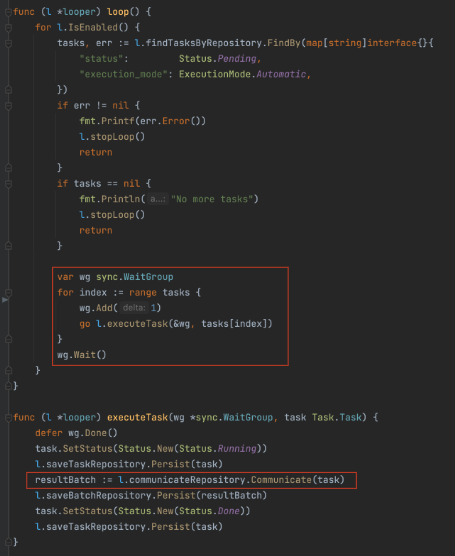
\includegraphics[height=0.3\textheight]{./part/Ejecucion/Seguimiento/Testing/img/Looper}
    \caption{testing looper.go detail}\label{fig:testingLooper}
\end{figure}

el punto clave de la figura \ref{fig:testingLooper} señalado en el recuadro rojo es el adaptador de comunicación GRPC es un adaptador experimental que debido a la inexperiencia en su uso está desarrollado de forma ineficiente. Hemos extraido toda la lógica posible a este servicio que es la parte core:

El adaptador puede tener múltiples errores inesperados, no conseguir comunicar con el servicio cliente, timeouts, malas implementaciones de la librería, pero se ha protegido al dominio de todo esto mediante una interfaz que garantiza que ante cualquier error se devuelve siempre un resultado. Lo único que quedaría por implementar y testear sería que el proceso no consiguiera terminar y se quedara la gorutine en un proceso infinito. para ello en el proceso de descubrimiento del lenguaje sabemos que hay un punto débil en el dominio. No hemos hehco uso de una herramienta de Golang que se conoce como context. que permite gestionar los timeouts de las gorutines evitando que que queden procesos hijos sin control.

Tengamos en cuenta que hemos extraido de toda la comunicación con el cliente una interfaz útil y única para comunicarnos, una lógica de negocio que entender en pocas lineas de código y explicar su funcionamiento, controlarlo y testearlo y aún así encontramos puntos débiles que mejorar en ese diseño. Si a esto le hubieramos sumado las lineas de codigo que hay detrás de la interfaz de comunicacion sería ingestionable. para cuantificar esto vamos a hacer una aproximación al diseño del test necesario para cubrir el adaptador de comunicacion

El código completo se encuentra en el repositorio github. Simplificando para esta explicación el pseudocódigo sería el siguiente

\begin{verbatim}
connection, err := grpc.Dial()
    serverStream:
        client.CallServerStream(request)
        responseStream.Recv()
    Bidirectional:
        client.CallBidirectional()
        async stream.Recv()
        async stream.Send()
        stream.CloseSend()
    ClientStream:
        client.CallClientStream()
        stream.Send
        stream.CloseAndRecv()
    Unary
        client.CallUnary()
connection.Close()
\end{verbatim}

vemos que hay mucha lógica junta, múltiples responsabilidades y por lo tanto no es un buen diseño. Como se demuestra mejor es intentando diseñar los tests. Para empezar extraer del código estas clases de equivalencia y factores no ha sido sencillo ya que hay multiples gestiones de errores dispersos por el código y es un código extenso 178 lineas. Esto ocurre en multitud de ocasiones, ya sea debido al tiempo, desconocimiento o mala praxis nos encontramos con códigos de esta magnitud. La arquitectura y todo este proceso lo que hace es protegernos de estas secciones sucias.

factores y posibles respuestas:

\begin{itemize}
    \item grpc.Dial(): err, connection
    \item client.CallServerStream(request): err,stream
    \item responseStream.Recv(): EOF,err,nil
    \item client.CallBidirectional(): error,stream
    \item stream.Recv(): EOF,err, result
    \item stream.Send(): EOF, nil,err
    \item stream.CloseSend() err,nil
    \item client.CallClientStream(): err, stream
    \item stream.Send: err, nil
    \item stream.CloseAndRecv(): err, nil
    \item client.CallUnary(): err,nil
    \item connection.Close(): err, nil
\end{itemize}

Si no entendieramos bien el concepto de clase de equivalencia podría llevarnos a un mal diseño de los tests o a hacerlo más complejo. Aunque hay factores que tiene tres respuestas posibles EOF y nil tienen que ir de la mano, significa que no ha habido error, primero obtienes un nil en el error y luego obtienes un error tipo EOF que significa que todo ha terminado correctamente. y luego tenemos cuando obtenmos un error distinto de EOF, si esto ocurre nos importa cuaántas veces haya ocurrido el caso sin error, será error igualmente. Con lo cual las clases de equivalencia serían

\begin{itemize}
    \item grpc.Dial(): err, connection
    \item client.CallServerStream(): err,stream
    \item responseStream.Recv(): nil\&EOF,err
    \item client.CallBidirectional(): error,stream
    \item stream.Recv(): nil\&EOF,err
    \item stream.Send(): nil\&EOF,err
    \item stream.CloseSend() err,nil
    \item client.CallClientStream(): err, stream
    \item stream.Send: err, nil
    \item stream.CloseAndRecv(): err, nil
    \item client.CallUnary(): err,nil
    \item connection.Close(): err, nil
\end{itemize}

para este caso tendríamos \[ 2^{12} = 4096 \] combinaciones posibles que pairwise reduce a 59 tests. aquí se ve la potencia del método. Volviendo posible un testing con ciertas garantías incluso en un código como el que nos ocupa.

\paragraph{Robustez ante nuevos desarrollo}

Uno de los puntos más relevantes de un proyecto de software es garantizar la viabilidad en la continuidad del desarrollo futuro; ya sea por mantenimiento o adición de nuevas características.

Para esto hay que tener en cuenta que uno de los factores más limitantes es la acumulación de conocimiento acerca del sistema en los ténicos. Tener un sistema que evite tener que conocer todo el proyecto en profundidad para realizar cambios es crítico. Uno de estos puntos es la infraestructura. El hecho de instalar el sistema en su modo para el desarrollo es en sí un reto. Instalar dependencias y garantizar que todo está funcional.

Por ello es importante, no sólo la documentación, si herramientas que levanten el sistema de forma automatizada y generalizada para cualquier dispositivo. A nuestra disposición tenemos Docker~\cref{par:Docker}, scripts y archivos Makefile.

Dentro de esos contendores Docker dispondremos de todas las herramientas ya instaladas para manejar el sistema sin tener que instalarlas en nuestra propia máquina.

Para este proyecto necesitaremos garantizar:

\begin{itemize}
    \item versión fija de golang para compilar los programas
    \item versión fija de la las librerias
    \item versión fija de la base de datos
    \item configuración del protocolo de comunicación entre sistemas
\end{itemize}

tendremos un archivo Makefile en cada programa para:

\begin{itemize}
    \item interactuar con el sistema de contenedores docker~\cref{par:Docker}
    \item interactuar con el protocolo GRPC~\cref{subsubsec:communications}
    \item interactuar con la base de datos~\cref{par:mysql}
\end{itemize}




